\documentclass[final]{beamer}
%\usetheme{chalmers}
% \usetheme{Custom}
% \usetheme{I6dv}
\usecolortheme{seahorse}
\usepackage[english]{babel}
\usepackage[T1]{fontenc}
% \usepackage{palatino}
\usepackage{DejaVuSans}
\usepackage{bbding}
\usepackage[sans]{dsfont}
\usepackage[orientation=portrait,size=a1,scale=2]{beamerposter}
 \usepackage[absolute,overlay]{textpos}
\usepackage{bold-extra}
% \usepackage{verbatim}
\usepackage{tikz}
% \usetikzlibrary{matrix}
\usepackage{calc}
% \usepackage[thicklines]{cancel}
% \usepackage{xcolor}
% \renewcommand{\CancelColor}{\color{red}}

% \beamerboxesrounded

% \setbeamercolor{block title}{fg=black,bg=gray!40}
% \setbeamercolor{block body}{fg=black,bg=gray!10}

% \newenvironment{colorblock}
% {
% \begin{beamerboxesrounded}[upper=upcol,lower=lowcol,shadow=true]}
% {\end{beamerboxesrounded}}


\newcommand{\cancel}[1]{%
    \tikz[baseline=(tocancel.base)]{
        \node[inner sep=0pt,outer sep=0pt] (tocancel) {#1};
        \draw[line width=10pt][red] (tocancel.south west) -- (tocancel.north east);
    }%
}%

% \setbeamertemplate{blocktitle}[default=center]
\setbeamertemplate{navigation symbols}{}

%\setbeamertemplate{blocks}[rounded][shadow=true]
% \setbeamercolor*{block body}{bg=blockBodyBackground,fg=grey}
% \setbeamercolor{block
% footer}{bg=blockFooterBackground,fg=blockFooterForeground}
\setbeamercolor{block title}{bg=blue!15}
%\setbeamerfont{block title}{size=\Large,series=\bf\sf}

\setbeamertemplate{frametitle}[default][center]


\title{Programming Logic}
\author{}
%\footer{~}
\date{}

\begin{document}
\begin{frame}{\rule{0}{2em}\Huge Programming Logic\vfill}
%\maketitle
\vfill
  \begin{minipage}[c]{1.0\linewidth}
    \begin{columns}
      \begin{column}{0.45\textwidth}%
        \begin{block}{Foundations and Logic}
          \vskip.75em
          \begin{columns}
            \begin{column}{0.45\textwidth}
              {\small The barber shaves all, and only those, who do
                not shave themselves.

                Who shaves the barber?
              }\\
              \begin{center}
                {\small $R = \{ X \mid X \notin X \}$\\
                  $R \notin R$?}
              \end{center}
            \end{column}
            \begin{column}{0.45\textwidth}
              \includegraphics[scale=.5]{russell.jpg}
%              {\tiny B.~Russell}
            \end{column}
          \end{columns}
          % A barber who shaves  the people who don't shave
          % themselves, and
        \end{block}
      \end{column}

      \begin{column}{.48\textwidth}
        \begin{block}{Constructive Mathematics}
          \vskip.75em
          \begin{center}
            \fbox{\huge \cancel{${A \lor \neg A}$}}
          \end{center}
          A mathematical object only exists by an explicit
          construction.
          \vskip4em
        \end{block}
        \vfill
      \end{column}
    \end{columns}
  \end{minipage}
  % \begin{block}{}
  % \end{block}
  % \vfill
   \vskip1em
  \begin{block}{Dependent Type Theory}
    \begin{itemize}
    \item Programming language and foundation of mathematics in one!
    \item Proving = programming
    \item Correctness by construction!
    \end{itemize}
    \begin{columns}
      \begin{column}{.45\textwidth-1ex}%
        \begin{block}{Agda \hfill {\small (made in Chalmers)}}

          \begin{center}
            Functional Programming
            $+$
            Dependent Types
          \end{center}

          \begin{minipage}{.45\textwidth-1ex}
            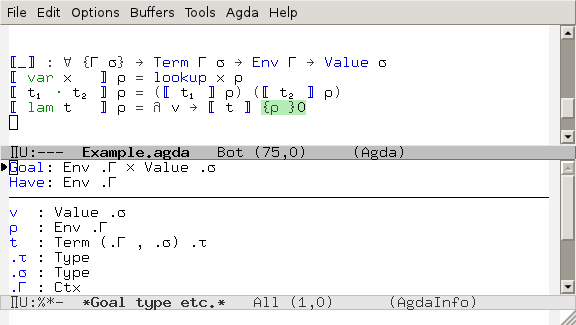
\includegraphics[scale=1.2]{emacs.png}
          \end{minipage}
        \end{block}

      \end{column}
      \begin{column}{.45\textwidth-1ex}%
        \begin{block}{Formalization}
          % Interactive theorem proving (with Coq \& Agda) o
          {\small Computer assisted verification of proofs and
            programs}
          \includegraphics[scale=2, angle=90]{fcolor.png}\\
          {\small How many colors are needed to color any map?}
        \end{block}

      \end{column}
    \end{columns}
    \begin{block}{Homotopy Type Theory}
      \begin{columns}
        \begin{column}{.25\textwidth-1ex}
          \includegraphics[scale=2]{donut.png}
        \end{column}
        \begin{column}{.65\textwidth-1ex}
          New foundation of mathematics: a connection between Computer
          Science, Geometry and Logic!
        \end{column}
      \end{columns}
    \end{block}

  \end{block}
\vfill
\end{frame}


\end{document}


%%% Local Variables: 
%%% mode: latex
%%% TeX-master: t
%%% End: 
